\documentclass[a4paper,11pt,titlepage]{jsarticle}
\usepackage{color}
% \title{核内αクラスター形成確率振幅の系統的分析}
% \author{6530-32-0490 上田永樹\thanks{京都大学大学院エネルギー科学研究科 エネルギー基礎科学専攻 修士課程}}
% \date{論文提出日 2021/01/31}


\usepackage{docmute}
\usepackage{braket}%ブラケット関係のやつ
\usepackage[dvipdfmx]{graphicx}%画像関係のやつ
\usepackage[dvipdfmx]{color}
\usepackage{here}%よくわからん
\usepackage{bm}%ベクトル関係のやつ
\usepackage{amsmath} %数学関係のやつ
\usepackage{listings} %プログラムソースのinclude
\usepackage{color}
% \usepackage{scalefnt}
 
\lstset{ 
  basicstyle={\ttfamily},
  identifierstyle={\small},
  commentstyle={\smallitshape},
  keywordstyle={\small\bfseries},
  ndkeywordstyle={\small},
  stringstyle={\small\ttfamily},
  frame={tb},
  breaklines=true, 
  columns=[l]{fullflexible},
  numbers=left,
  xrightmargin=0zw,
  xleftmargin=3zw,
  numberstyle={\scriptsize},
  stepnumber=1,
  numbersep=1zw,
  lineskip=-0.5ex
} %listingsの設定

\numberwithin{equation}{section} %上手い式の数振り
\setcounter{tocdepth}{3} %subsubsectionまで目次に表示

 

\begin{document}

% input1st
  \section{序論}
  \subsection{高強度レーザー技術の進展}

  1960年代、T.H.Maimanがルビーを用いた固体レーザーの発振に成功した\cite{ft1}ことを皮切りに、レーザー技術は発展し続け、
  1964年にはL.E.Hargroveが開発したモードロックレーザーによってフェムト秒レーザーの発振が達成された\cite{ft2}。
  レーザー発振時の結晶や光学機器の損傷などの問題から、レーザーの高強度化技術は一時停滞していたが、
  1985年に高強度レーザーを得るための極短パルス増幅法である、チャーブパルス増幅法(Chirped Pulse Amplification、CPA)\cite{ft3}
  が開発されたことでレーザーの集光強度(単位:W/cm$^{2}$)は飛躍的に向上し、特に、集光強度が10$^{18}$ W/cm$^{2}$を超えるようになったことで、
  レーザーは電子を光速に近い速度(~0.5 MeV)にまで加速させることが可能となり、電子の相対論領域を扱う新領域の開拓が実現した(図1参照)。
  この功績からG.Mourouらは、2018年にノーベル物理学賞を受賞している。

  \begin{table}[H]
    \caption{レーザーの一覧}
    \centering
    \scalebox{0.85}{
      \begin{tabular}{lccccc} \hline \hline
        \multicolumn{5}{c}{レーザーの一覧} \\ \hline
        レーザー & 集光強度 & パルス幅 & 最大エネルギー & 波長 & 出力 \\ \hline 
        激光 XII(日) & $\sim 1\times 10^{19}\ \mathrm{W/cm^{2}}$ 
        & 0.1 $\sim$ 0.4 ns & 250 $\sim$ 1000 J & 527 or 1053 nm & 1 PW \\
        NIF(米) & $\sim 1\times 10^{16}\ \mathrm{W/cm^{2}}$  & 20 ns & 1.8J & 1053 nm & 500 TW \\ \hline
        LFEX(日)  & $ \sim 1\times 10^{19}\ \mathrm{W/cm^{2}}$ 
        & $0.5 \sim 20$ ps 
        & 2.5 kJ & 1053 nm & 2 PW \\ 
        OMEGA EP(米) & $ \sim 6 \times 10^{19}\ \mathrm{W/cm^{2}}$ 
        & $0.7 \sim 100$ ps 
        & 0.5 $\sim$ 2.3 kJ & 1053 nm & 不明 \\ \hline
        J-KAREN(日) & $ \sim 1\times 10^{22}\ \mathrm{W/cm^{2}}$ & 40 fs 
        & 30 J & 810 nm & 1 PW \\ %\hline \hline
        ELI(羅) & $\sim 1\times 10^{23}\ \mathrm{W/cm^{2}}$  & $\sim 17$ fs
        & $\sim$ 34 J & 800 $\sim$ 1030 nm & $\sim$ PW \\ \hline \hline
    \end{tabular}
    }
  \end{table}

  最近では、量子科学技術研究開発機構・関西光科学研究所のJ-KAREN-Pレーザー
  \cite{Kiriyama2015, AlexOE2017,  Kiriyama2018,Kiriyama2020}などが
  レーザーの最大集光強度$10^{21-22}\ \mathrm{W/cm^{2}}$領域の
  フェムト秒極短パルス高強度レーザーを実現している。
  このような高出力レーザーを物質に照射することで、物質はレーザーのパルス時間スケール(フェムト秒オーダ)で瞬時に電離してプラズマ化するとともに、
  発生した多数の電子がレーザー光の光圧によりレーザー伝播方向に光速に近い速度にまで加速される。このような電子の相対論領域での運動により、
  プラズマ中にはメガアンペア(MA)に達する大電流が駆動され、中性子パルサーに匹敵する数10キロテスラ(kT)の磁場が生成するとともに、
  イオンと電子との電荷分離に起因して数10TV/mに達する電場が形成される。
  この電場はイオンを数10 MeV/u(核子当たり)にまで加速させる。
  すなわち、圧力が太陽の中心部の圧力(2000億気圧)の1/10に迫る、100億気圧オーダの高エネルギー密度プラズマが実験室レベルで生成可能である。

  \begin{figure}[H]
    \begin{center}
      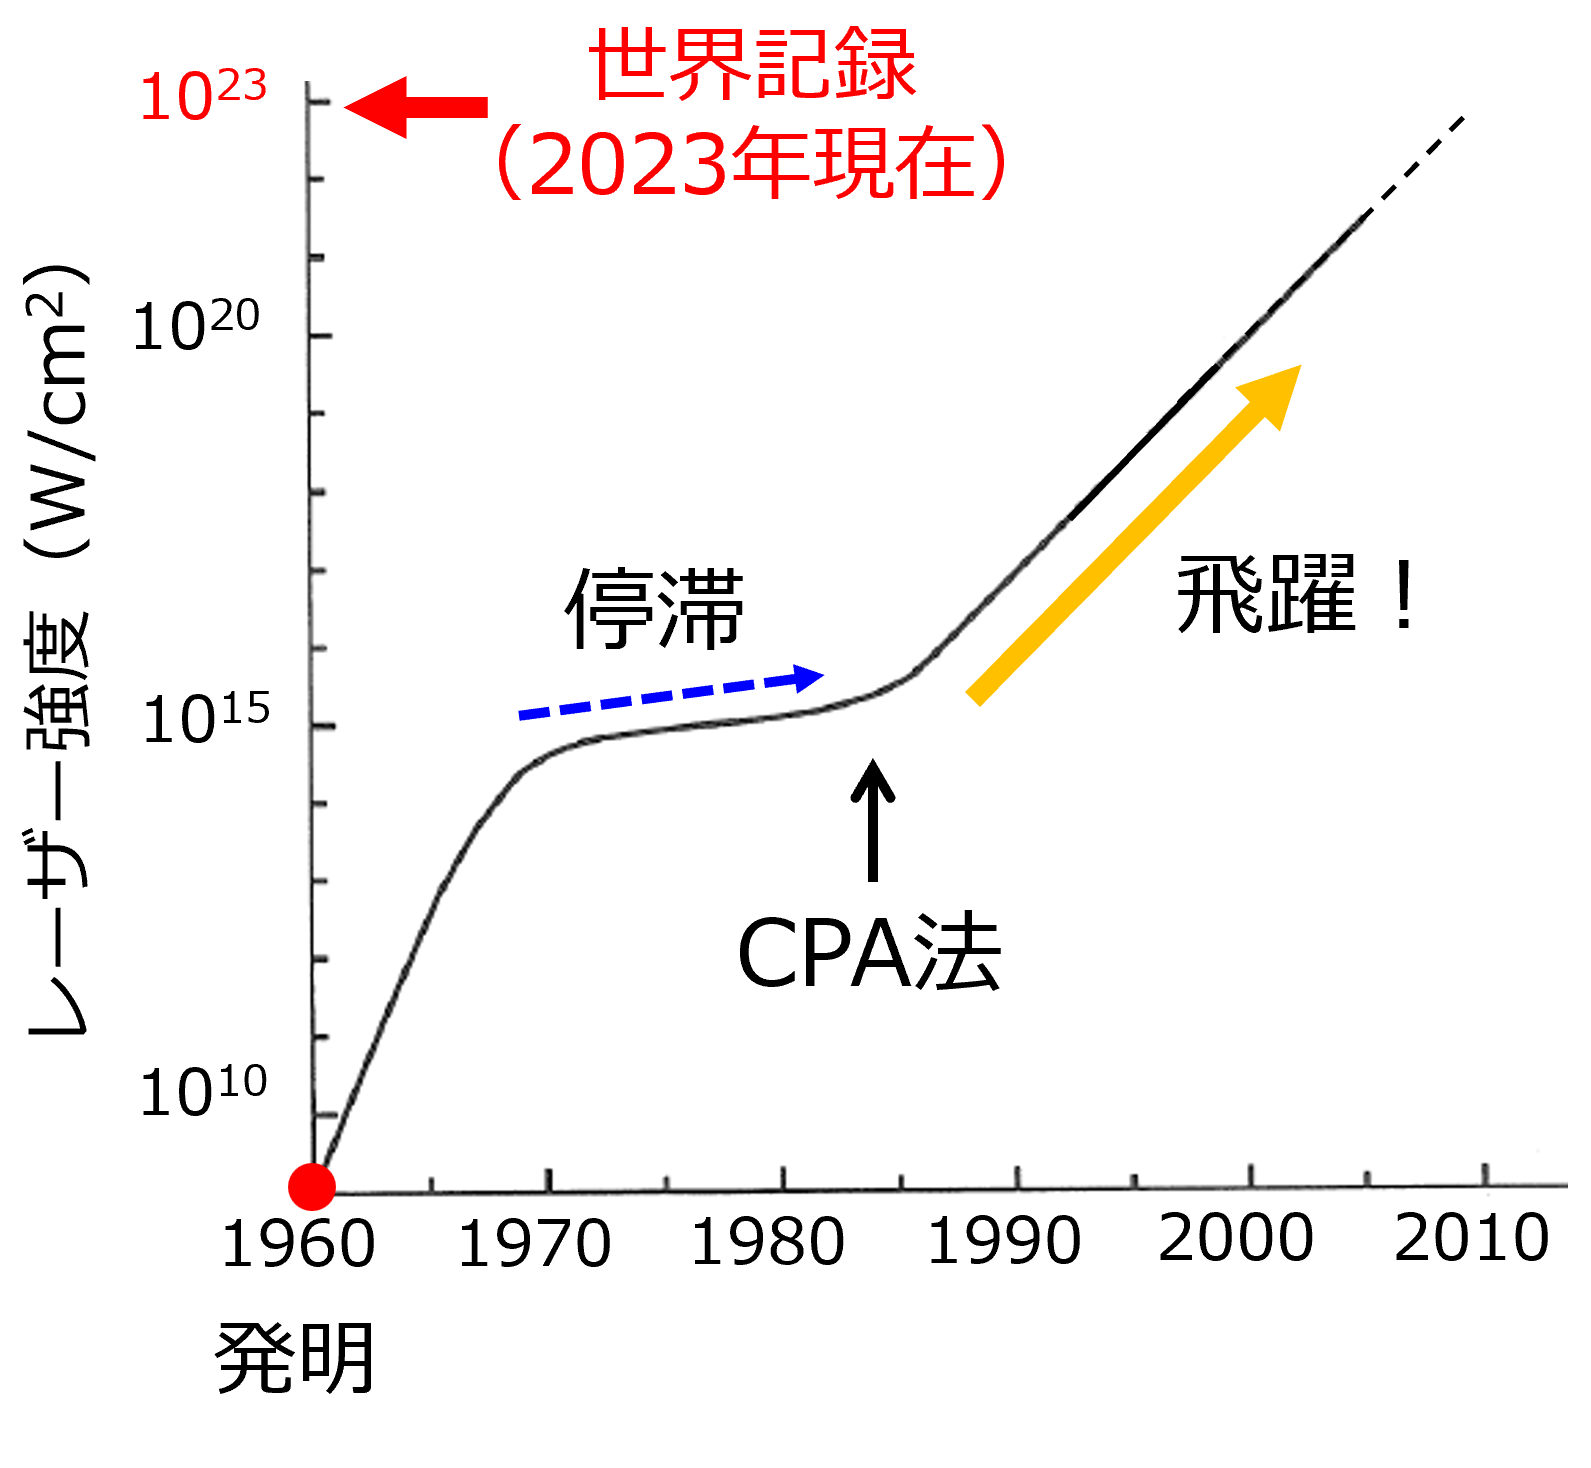
\includegraphics[scale=0.4]{./image/1-laser.png}
      \label{fig:1}
      \caption{高強度レーザー技術の発展。横軸は西暦、
      縦軸左は達成されたレーザーの最大集光強度(単位:W/cm$^2$)を示している。
      1985年のチャープパルス増幅法(Chirped Pulse Amplification,CPA法)の開発により、
      レーザー強度は飛躍的に増大している。
      縦軸右はレーザーにより電子が加速された際に得られる電子エネルギー(単位:eV(電子ボルト))を
      表しており、集光強度が10$^{18}$ W/cm$^{2}$で電子は相対論領域(速さ$v$~$c$、$c$:光速)となる。}
    \end{center}
  \end{figure}

  \subsection{医療・産業・学術への応用}
  このような宇宙レベルの超強電磁場を伴う高エネルギー密度プラズマは、医療応用を目指した小型イオン源の開発や慣性核融合炉の実現や新物質創出に向けた中性子源・高輝度x線源、
  高エネルギー宇宙線の生成起源やフェルミ加速機構・ワイベル不安定性による磁場増幅機構などの解明に向けた実験室宇宙物理など、
  様々な医療・産業・学術応用が期待されている。
  \par
  
  
  

  高強度レーザーを照射する物質としては、これまで主に固体薄膜・高圧ガス等が用いられており、
  これらにレーザーを照射することで、物質との境界層に高エネルギー密度プラズマを生成することが可能である。
  一方で、このようにして生成されたプラズマは、慣性時間$\tau_0 \sim L/C_s$
  (\textit{L}:プラズマのサイズ、$C_s$:音速)で飛散してしまうため、応用研究の対象が
  この時間スケールに収まる現象に限定される。

  \subsection{構造性媒質}

  こうした背景のもと、我々は、物質にレーザー波長以下のサブ$\mu$mオーダの微細構造を付与した
  構造性媒質を照射ターゲットとして選択し、これに高強度レーザーを照射する実験を行ったところ、
  % エネルギー吸収率の増大に関して
  % 構造性媒質の形状に起因する多彩な現象の創出(音速の制御→慣性時間の伸長、準定常磁場生成)
  
  \subsection{研究目的}

  \subsection{本論文の構成}

  2章では高強度レーザーと物質の相互作用を支配する物理現象について説明する。
  はじめにレーザー強度とパラメータについて記述し、それを踏まえ相対論領域(高強度レーザー領域)での電子の特徴的な運動について記述する。
  次にプラズマ内部への電磁波伝搬について記述する。
  また、今回ロッドの基本性質を明らかにするために用いたエネルギー保存則と、導体極板間での電磁波伝搬についても記述する。
  3章ではシミュレーションで扱う粒子コードの概要と各パラメータの規格化などについて記述する。
  4章では、今回行ったシミュレーション結果を記載し、その考察をする。
  側面照射を模擬した2Dシミュレーションでは、ロッド径が慣性時間伸長に寄与しうるパラメータであるかの検証、
  上面照射を模擬した2Dシミュレーションでは、基盤ターゲット及び構造を付与したターゲットにおける物理過程の差異について考察する。
  また、ここではエネルギー保存則を任意の分割領域に適応することで、構造性媒質の性質を明らかにする。
  最後に3Dシミュレーションを用いて、上述のシミュレーション結果を大域的に説明する。

% input1ed
\begin{thebibliography}{99}
\bibitem{Kiriyama2015}
H. Kiriyama $et\ al.,$ IEEE J. Sel. Top. Quantum Phys. {\bf 21}(1), 232-249 (2015). 
\bibitem{AlexOE2017}
A. S. Pirozhkov $et\ al.,$ Opt. Express {\bf 25}(17), 20486 (2017). 
\bibitem{Kiriyama2018}
H. Kiriyama $et\ al.,$ Optics Letters {\bf 43}, 2595 (2018).
\bibitem{Kiriyama2020}
H. Kiriyama $et\ al.,$ Optics Letters {\bf 45}, 1100 (2020).
\end{thebibliography}
\newpage

\end{document}

